% Chapter 8: Security Analysis
\chapter{Security Analysis}
\label{ch:security}

This chapter provides a comprehensive security analysis of \tprotocol{}, including formal threat modeling, cryptographic primitive analysis, attack scenarios, and deployment recommendations.

\section{Security Philosophy}
\label{sec:security-philosophy}

\tprotocol{} follows a \textbf{defense-in-depth} approach with multiple layers of protection:

\begin{enumerate}
    \item \textbf{Cryptographic Layer}: Strong signature schemes prevent forgery
    \item \textbf{Protocol Layer}: Nonces and deadlines prevent replay
    \item \textbf{Blockchain Layer}: On-chain verification ensures finality
    \item \textbf{Transport Layer}: HTTPS protects data in transit
\end{enumerate}

\begin{infobox}[Core Security Principle]
\tprotocol{} is designed so that a malicious Facilitator cannot steal user funds. The Facilitator can only settle payments to the \field{payTo} address specified in the cryptographically signed authorization. This is verified on-chain by the token contract.
\end{infobox}

\section{Formal Threat Model}
\label{sec:threat-model-formal}

\subsection{Adversary Capabilities}

We consider adversaries with the following capabilities:

\begin{table}[h]
\centering
\caption{Adversary Capability Matrix}
\label{tab:adversary-capabilities}
\begin{tabular}{lp{8cm}}
\toprule
\textbf{Capability} & \textbf{Description} \\
\midrule
Network Access & Can observe and modify network traffic (MitM) \\
API Access & Can send arbitrary requests to public APIs \\
Prior Payments & Has access to previously completed payment data \\
Blockchain Access & Can submit transactions to public blockchains \\
\bottomrule
\end{tabular}
\end{table}

\subsection{Adversary Limitations}

The security model assumes adversaries \textbf{cannot}:

\begin{itemize}
    \item Compute discrete logarithms (break ECDSA/Ed25519)
    \item Find hash collisions (break Keccak-256/SHA-256)
    \item Compromise the user's private key
    \item Perform 51\% attacks on supported blockchains
\end{itemize}

\subsection{Threat Categories}

\begin{figure}[ht]
\centering
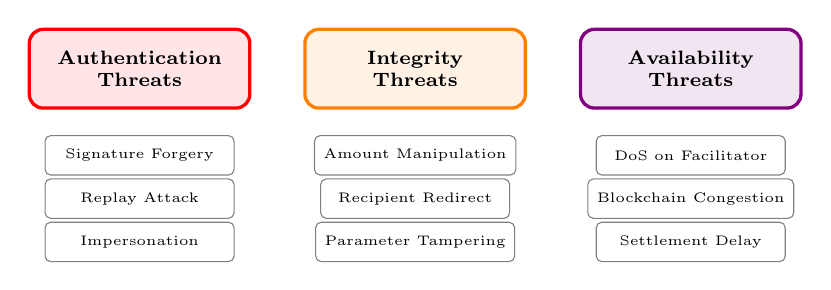
\begin{tikzpicture}[
    category/.style={
        rectangle,
        rounded corners=5pt,
        minimum width=2.8cm,
        minimum height=1cm,
        line width=1.2pt,
        font=\bfseries\scriptsize,
        align=center
    },
    subcategory/.style={
        rectangle,
        rounded corners=2pt,
        minimum width=2.4cm,
        minimum height=0.5cm,
        draw=gray,
        fill=white,
        font=\tiny,
        align=center
    }
]

% Main categories
\node[category, draw=red, fill=red!10] (auth) at (0,0) {Authentication\\Threats};
\node[category, draw=orange, fill=orange!10] (integrity) at (3.5,0) {Integrity\\Threats};
\node[category, draw=violet, fill=violet!10] (availability) at (7,0) {Availability\\Threats};

% Subcategories for Authentication
\node[subcategory] at (0,-1.1) {Signature Forgery};
\node[subcategory] at (0,-1.65) {Replay Attack};
\node[subcategory] at (0,-2.2) {Impersonation};

% Subcategories for Integrity
\node[subcategory] at (3.5,-1.1) {Amount Manipulation};
\node[subcategory] at (3.5,-1.65) {Recipient Redirect};
\node[subcategory] at (3.5,-2.2) {Parameter Tampering};

% Subcategories for Availability
\node[subcategory] at (7,-1.1) {DoS on Facilitator};
\node[subcategory] at (7,-1.65) {Blockchain Congestion};
\node[subcategory] at (7,-2.2) {Settlement Delay};

\end{tikzpicture}
\caption{Threat category taxonomy}
\label{fig:threat-taxonomy}
\end{figure}

\section{Attack Analysis}
\label{sec:attack-analysis}

This section provides detailed analysis of specific attack vectors and their mitigations.

\subsection{Replay Attacks}

\begin{securitybox}[Replay Attack Definition]
An adversary captures a valid payment authorization and attempts to reuse it for additional payments.
\end{securitybox}

\subsubsection{Attack Vector}

\begin{enumerate}
    \item Adversary observes valid \code{PaymentPayload} from Client to Server
    \item Adversary saves the payload including the signature
    \item Adversary submits the same payload to a different Server or the same Server later
\end{enumerate}

\subsubsection{Mitigations}

\tprotocol{} employs three-layer replay protection:

\begin{table}[h]
\centering
\caption{Replay Attack Mitigations}
\label{tab:replay-mitigations}
\begin{tabular}{llp{5.5cm}}
\toprule
\textbf{Layer} & \textbf{Mechanism} & \textbf{Protection} \\
\midrule
Temporal & \field{validBefore} & Authorization expires after deadline \\
Uniqueness & \field{nonce} & 32-byte random, checked on-chain \\
Domain & EIP-712 Domain & Chain and contract-specific binding \\
\bottomrule
\end{tabular}
\end{table}

\begin{algorithm}[H]
\caption{Replay Protection Verification}
\label{alg:replay-protection}
\SetKwInOut{Input}{Input}
\SetKwInOut{Output}{Output}
\Input{Authorization $A$, Current time $t$}
\Output{Boolean (protected)}

\BlankLine
\tcp{Temporal check}
\If{$t > A.validBefore$}{
    \Return{true} \tcp{Expired, cannot be replayed}
}

\BlankLine
\tcp{Nonce check (on-chain)}
$used \gets \text{authorizationState}(A.from, A.nonce)$\;
\If{$used$}{
    \Return{true} \tcp{Already used, cannot be replayed}
}

\BlankLine
\tcp{Domain check (signature verification)}
$domain \gets \{chainId, verifyingContract\}$\;
\If{$domain \neq A.signedDomain$}{
    \Return{true} \tcp{Wrong chain/contract, invalid signature}
}

\Return{false} \tcp{Valid, could potentially be replayed}
\end{algorithm}

\subsection{Signature Forgery}

\begin{securitybox}[Signature Forgery Definition]
An adversary attempts to create a valid authorization signature without possessing the private key.
\end{securitybox}

\subsubsection{Attack Resistance}

\begin{theorem}[Signature Unforgeability]
Under the Elliptic Curve Discrete Logarithm Problem (ECDLP) assumption, an adversary cannot forge a valid EIP-3009 authorization signature in probabilistic polynomial time.
\end{theorem}

\begin{proof}[Proof Sketch]
EIP-3009 uses ECDSA signatures over the secp256k1 curve. The security reduces to:

\begin{enumerate}
    \item \textbf{ECDLP Hardness}: Given $G$ and $kG$, computing $k$ is computationally infeasible
    \item \textbf{EIP-712 Binding}: The typed data hash binds all authorization parameters
    \item \textbf{On-chain Verification}: \code{ecrecover} extracts signer from signature
\end{enumerate}

Any signature forgery would imply either:
\begin{itemize}
    \item Solving ECDLP (contradicts assumption)
    \item Finding hash collision (Keccak-256 is collision-resistant)
    \item Exploiting \code{ecrecover} (extensively audited)
\end{itemize}
\end{proof}

\subsection{Man-in-the-Middle (MitM)}

\subsubsection{Attack Vector}

\begin{enumerate}
    \item Adversary intercepts 402 response from Server
    \item Modifies \field{payTo} to adversary's address
    \item Client signs payment to adversary instead of Server
\end{enumerate}

\subsubsection{Mitigations}

\begin{enumerate}
    \item \textbf{HTTPS Requirement}: All \tprotocol{} traffic MUST use TLS 1.2+
    \item \textbf{Certificate Verification}: Clients MUST verify server certificates
    \item \textbf{Signed Parameters}: All payment parameters are included in signature
\end{enumerate}

\begin{warningbox}[Client Implementation Requirement]
Clients MUST verify the \field{payTo} address belongs to the expected recipient before signing. This is typically done by matching against the request domain or a trusted list.
\end{warningbox}

\subsection{Double Spending}

\subsubsection{Attack Vector}

\begin{enumerate}
    \item Client creates authorization for payment
    \item Server verifies and serves content
    \item Client attempts to spend same funds elsewhere before settlement
\end{enumerate}

\subsubsection{Mitigations}

\begin{enumerate}
    \item \textbf{Balance Check}: Facilitator verifies sufficient balance during \code{/verify}
    \item \textbf{Prompt Settlement}: Settlement typically occurs within seconds
    \item \textbf{Blockchain Finality}: Once settled, transaction is irreversible
\end{enumerate}

\begin{table}[h]
\centering
\caption{Double Spend Window by Chain}
\label{tab:double-spend-window}
\begin{tabular}{lll}
\toprule
\textbf{Chain} & \textbf{Finality} & \textbf{Risk Window} \\
\midrule
Base/Optimism & $\sim$2 seconds & Low \\
Arbitrum & $\sim$1 second & Low \\
Solana & $\sim$0.4 seconds & Very Low \\
TON & $\sim$5 seconds & Low \\
Ethereum L1 & $\sim$13 minutes & Moderate \\
\bottomrule
\end{tabular}
\end{table}

\subsection{Insufficient Payment Attack}

\subsubsection{Attack Vector}

\begin{enumerate}
    \item Server requires payment of $X$ tokens
    \item Client signs authorization for $X - \epsilon$ tokens
    \item Client attempts to claim full value of service
\end{enumerate}

\subsubsection{Mitigations}

\begin{enumerate}
    \item \textbf{Amount Verification}: Facilitator checks $authorization.value \geq requirements.amount$
    \item \textbf{Exact Match}: For \code{exact} scheme, values must match precisely
    \item \textbf{Server Validation}: Server re-verifies before serving content
\end{enumerate}

\subsection{Wrong Recipient Attack}

\subsubsection{Attack Vector}

\begin{enumerate}
    \item Malicious Facilitator intercepts payment request
    \item Modifies \field{payTo} in settlement call
    \item Redirects funds to attacker's wallet
\end{enumerate}

\subsubsection{Mitigations}

\begin{theorem}[Recipient Binding]
A correctly signed EIP-3009 authorization cannot be settled to any address other than the \field{to} address included in the signed data.
\end{theorem}

\begin{proof}
The EIP-712 typed data includes the \field{to} parameter in the hash:

\begin{lstlisting}[language=typescript]
const types = {
  TransferWithAuthorization: [
    { name: "from", type: "address" },
    { name: "to", type: "address" },    // Bound in signature
    { name: "value", type: "uint256" },
    // ...
  ]
};
\end{lstlisting}

The token contract verifies:
\begin{lstlisting}[language=solidity]
require(
    ecrecover(hash, v, r, s) == from,
    "Invalid signature"
);
// If signature valid, 'to' is cryptographically bound
\end{lstlisting}
\end{proof}

\section{Cryptographic Security}
\label{sec:crypto-security}

\subsection{Signature Algorithms}

\begin{table}[h]
\centering
\caption{Cryptographic Primitive Security Levels}
\label{tab:crypto-security}
\begin{tabular}{llll}
\toprule
\textbf{Chain} & \textbf{Algorithm} & \textbf{Key Size} & \textbf{Security Level} \\
\midrule
EVM & ECDSA secp256k1 & 256 bits & 128 bits \\
Solana & Ed25519 & 256 bits & 128 bits \\
TON & Ed25519 & 256 bits & 128 bits \\
TRON & ECDSA secp256k1 & 256 bits & 128 bits \\
\bottomrule
\end{tabular}
\end{table}

\subsection{Hash Functions}

\begin{table}[h]
\centering
\caption{Hash Function Properties}
\label{tab:hash-security}
\begin{tabular}{llll}
\toprule
\textbf{Function} & \textbf{Output} & \textbf{Collision Resistance} & \textbf{Usage} \\
\midrule
Keccak-256 & 256 bits & 128 bits & EIP-712 domain hash \\
SHA-256 & 256 bits & 128 bits & Solana, TON, TRON \\
\bottomrule
\end{tabular}
\end{table}

\subsection{Nonce Generation}

\begin{securitybox}[Nonce Requirements]
Nonces MUST be generated using a cryptographically secure random number generator (CSPRNG). Using predictable or sequential nonces enables attack vectors.
\end{securitybox}

\begin{lstlisting}[language=typescript,caption={Secure nonce generation}]
import { randomBytes } from 'crypto';

// Good: Cryptographically secure random bytes
const nonce = '0x' + randomBytes(32).toString('hex');

// Bad: Predictable
const nonce = Date.now().toString(16).padStart(64, '0');

// Bad: Sequential
const nonce = (lastNonce + 1n).toString(16).padStart(64, '0');
\end{lstlisting}

\section{Facilitator Security}
\label{sec:security-facilitator}

The Facilitator is a critical component that handles payment settlement. This section details its security requirements.

\subsection{Security Architecture}

\begin{figure}[ht]
\centering
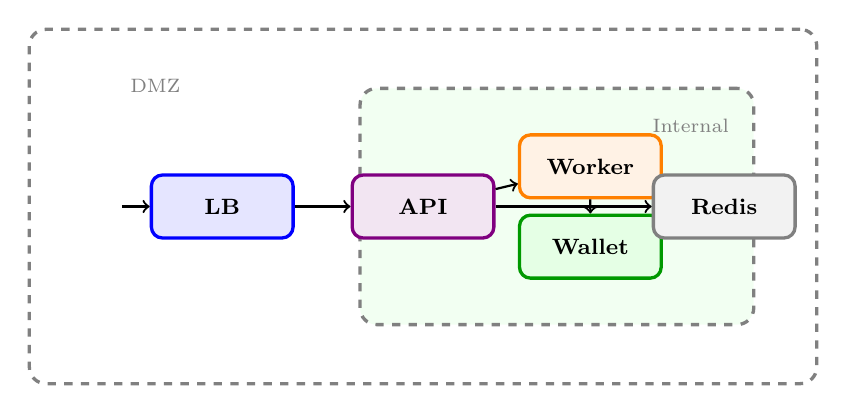
\begin{tikzpicture}[scale=0.85,
    component/.style={
        rectangle,
        rounded corners=4pt,
        minimum width=1.8cm,
        minimum height=0.8cm,
        line width=1.2pt,
        font=\footnotesize\bfseries,
        align=center
    },
    boundary/.style={
        rectangle,
        rounded corners=6pt,
        draw=gray,
        dashed,
        line width=1.2pt
    }
]

% External boundary
\node[boundary, minimum width=10cm, minimum height=4.5cm] at (0,0) {};
\node[font=\scriptsize, gray] at (-4,1.8) {DMZ};

% Internal boundary
\node[boundary, minimum width=5cm, minimum height=3cm, fill=green!5] at (2,0) {};
\node[font=\scriptsize, gray] at (4,1.2) {Internal};

% Components
\node[component, draw=blue, fill=blue!10] (lb) at (-3,0) {LB};
\node[component, draw=violet, fill=violet!10] (api) at (0,0) {API};
\node[component, draw=orange, fill=orange!10] (worker) at (2.5,0.6) {Worker};
\node[component, draw=green!60!black, fill=green!10] (wallet) at (2.5,-0.6) {Wallet};
\node[component, draw=gray, fill=gray!10] (redis) at (4.5,0) {Redis};

% Arrows
\draw[->, thick] (-4.5,0) -- (lb);
\draw[->, thick] (lb) -- (api);
\draw[->, thick] (api) -- (worker);
\draw[->, thick] (worker) -- (wallet);
\draw[->, thick] (api) -- (redis);

\end{tikzpicture}
\caption{Facilitator security architecture}
\label{fig:security-facilitator-architecture}
\end{figure}

\subsection{Hot Wallet Security}

\begin{warningbox}[Hot Wallet Risk]
The Facilitator hot wallet contains funds for gas payment. While it cannot access user funds, compromising this wallet results in loss of operational capacity.
\end{warningbox}

\subsubsection{Security Measures}

\begin{enumerate}
    \item \textbf{Minimum Balance}: Keep only funds necessary for gas
    \item \textbf{Monitoring}: Real-time alerts for unusual activity
    \item \textbf{Key Storage}: Use HSM or secure enclave where possible
    \item \textbf{Rotation}: Periodic key rotation
    \item \textbf{Separation}: Different wallets per environment
\end{enumerate}

\begin{lstlisting}[language=golang,caption={Secure key loading example}]
func loadPrivateKey() (*ecdsa.PrivateKey, error) {
    // Option 1: Environment variable (basic)
    keyHex := os.Getenv("PRIVATE_KEY")

    // Option 2: Secret manager (recommended)
    keyHex, err := vault.GetSecret("facilitator/evm-key")
    if err != nil {
        return nil, err
    }

    // Option 3: HSM (production)
    key, err := hsm.GetSigningKey("facilitator-key-id")
    if err != nil {
        return nil, err
    }

    return key, nil
}
\end{lstlisting}

\subsection{API Security}

\begin{table}[h]
\centering
\caption{Facilitator API Security Controls}
\label{tab:api-security}
\begin{tabular}{lp{7cm}}
\toprule
\textbf{Control} & \textbf{Description} \\
\midrule
Rate Limiting & 1000 req/60s per IP (configurable) \\
API Key Auth & Required for settlement endpoints \\
HTTPS Only & TLS 1.2+ mandatory \\
Input Validation & Strict schema validation on all inputs \\
CORS Policy & Configurable origin restrictions \\
Request Logging & Full audit trail of all operations \\
\bottomrule
\end{tabular}
\end{table}

\subsection{Denial of Service Protection}

\begin{enumerate}
    \item \textbf{Rate Limiting}: Per-IP and per-API-key limits
    \item \textbf{Request Size Limits}: Maximum payload size enforced
    \item \textbf{Timeout Configuration}: Aggressive timeouts on all operations
    \item \textbf{Circuit Breaker}: Automatic degradation under load
    \item \textbf{Geographic Distribution}: CDN and edge deployment
\end{enumerate}

\section{Chain-Specific Security}
\label{sec:chain-security}

\subsection{EVM Security Considerations}

\begin{securitybox}[EVM-Specific Checks]
\begin{itemize}
    \item Verify \field{chainId} in EIP-712 domain matches target network
    \item Check \field{verifyingContract} is the expected token address
    \item Validate \field{validBefore} is reasonable (not too far in future)
    \item Use cryptographically random 32-byte nonces
\end{itemize}
\end{securitybox}

\subsection{Solana Security Considerations}

\begin{securitybox}[Solana-Specific Checks]
The Facilitator MUST enforce:
\begin{enumerate}
    \item Exactly 3 instructions (ComputeBudget x2, TransferChecked)
    \item Fee payer NOT in any instruction accounts
    \item Compute unit price $\leq$ 5 lamports/CU
    \item Destination is correct ATA PDA
    \item Amount exactly matches requirements
\end{enumerate}
\end{securitybox}

\begin{lstlisting}[language=golang,caption={Solana security validation}]
func validateSolanaTransaction(tx *solana.Transaction, req *Requirements) error {
    // Check instruction count
    if len(tx.Message.Instructions) != 3 {
        return ErrInvalidInstructionCount
    }

    // Validate fee payer safety
    feePayer := tx.Message.AccountKeys[0]
    for _, inst := range tx.Message.Instructions {
        for _, acc := range inst.Accounts {
            if tx.Message.AccountKeys[acc] == feePayer {
                return ErrFeePayerInInstruction
            }
        }
    }

    // Validate compute price
    computePrice := extractComputePrice(tx)
    if computePrice > maxComputePrice {
        return ErrComputePriceTooHigh
    }

    return nil
}
\end{lstlisting}

\subsection{TON Security Considerations}

\begin{itemize}
    \item Validate Ed25519 signature over the BOC (Bag of Cells)
    \item Verify workchain ID is 0 (basechain)
    \item Check Jetton master contract matches expected USDT
    \item Validate sender wallet address computation
\end{itemize}

\subsection{TRON Security Considerations}

\begin{itemize}
    \item Validate Base58Check address format
    \item Verify contract is official USDT (\code{TR7NHqjeKQxGTCi8q8ZY4pL8otSzgjLj6t})
    \item Check sufficient energy for transaction
    \item Validate protobuf transaction structure
\end{itemize}

\section{Deployment Security}
\label{sec:deployment-security}

\subsection{Container Security}

\begin{lstlisting}[language=yaml,caption={Docker security configuration}]
version: '3.8'
services:
  facilitator:
    image: t402/facilitator:2.0.0
    security_opt:
      - no-new-privileges:true
    read_only: true
    tmpfs:
      - /tmp:noexec,nosuid,size=64M
    cap_drop:
      - ALL
    cap_add:
      - NET_BIND_SERVICE
    user: "1000:1000"
    networks:
      - internal
\end{lstlisting}

\subsection{Network Security}

\begin{enumerate}
    \item \textbf{Internal Network}: Service-to-service communication isolated
    \item \textbf{Reverse Proxy}: Only Caddy/Nginx exposed externally
    \item \textbf{Firewall Rules}: Whitelist only required ports
    \item \textbf{TLS Termination}: At edge, internal traffic optional
\end{enumerate}

\subsection{Secret Management}

\begin{table}[h]
\centering
\caption{Secret Management Requirements}
\label{tab:secrets}
\begin{tabular}{lll}
\toprule
\textbf{Secret} & \textbf{Storage} & \textbf{Rotation} \\
\midrule
Private Keys & HSM / Vault & 90 days \\
API Keys & Vault / Env & 30 days \\
Database Passwords & Vault & 90 days \\
TLS Certificates & ACME Auto & 90 days (Let's Encrypt) \\
\bottomrule
\end{tabular}
\end{table}

\section{Incident Response}
\label{sec:incident-response}

\subsection{Severity Classification}

\begin{table}[h]
\centering
\caption{Security Incident Severity Levels}
\label{tab:severity}
\begin{tabular}{llll}
\toprule
\textbf{Severity} & \textbf{Initial Response} & \textbf{Resolution} & \textbf{Example} \\
\midrule
Critical & 24 hours & 7 days & Private key leak \\
High & 48 hours & 30 days & Auth bypass \\
Medium & 72 hours & Next release & XSS vulnerability \\
Low & 7 days & Best effort & Minor info leak \\
\bottomrule
\end{tabular}
\end{table}

\subsection{Response Procedure}

\begin{enumerate}
    \item \textbf{Detection}: Automated monitoring or external report
    \item \textbf{Containment}: Isolate affected systems
    \item \textbf{Investigation}: Determine scope and impact
    \item \textbf{Eradication}: Remove threat
    \item \textbf{Recovery}: Restore services
    \item \textbf{Post-mortem}: Document and improve
\end{enumerate}

\section{Security Audit Status}
\label{sec:audit-status}

\subsection{Completed Audits}

\begin{table}[h]
\centering
\caption{Security Audit History}
\label{tab:audits}
\begin{tabular}{llll}
\toprule
\textbf{Component} & \textbf{Auditor} & \textbf{Date} & \textbf{Status} \\
\midrule
Protocol Design & Internal & 2024 Q4 & Complete \\
SDK Code Review & Internal & 2025 Q1 & Complete \\
External Audit & TBD & Planned & Pending \\
\bottomrule
\end{tabular}
\end{table}

\subsection{Continuous Security Measures}

\begin{itemize}
    \item \textbf{Dependency Scanning}: Dependabot, govulncheck, npm audit
    \item \textbf{Container Scanning}: Trivy in CI/CD
    \item \textbf{Secret Scanning}: GitHub secret scanning enabled
    \item \textbf{SBOM Generation}: Per-release software bill of materials
\end{itemize}

\section{Responsible Disclosure}
\label{sec:disclosure}

\subsection{Reporting Channels}

\begin{itemize}
    \item \textbf{GitHub Security Advisories}: Preferred method
    \item \textbf{Email}: \code{security@t402.io}
\end{itemize}

\section{Summary}
\label{sec:security-summary}

\begin{table}[h]
\centering
\caption{Security Property Summary}
\label{tab:security-summary}
\begin{tabular}{lp{8cm}}
\toprule
\textbf{Property} & \textbf{Guarantee} \\
\midrule
Non-custodial & Facilitator cannot access user funds \\
Recipient Binding & Payments can only go to signed \field{payTo} \\
Replay Protection & Nonces + deadlines + domain separation \\
Signature Security & 128-bit security level (ECDSA/Ed25519) \\
Settlement Finality & Blockchain consensus guarantees \\
\bottomrule
\end{tabular}
\end{table}
